
\documentclass[a4paper,11pt]{article}
\usepackage[a4paper, margin=8em]{geometry}

% usa i pacchetti per la scrittura in italiano
\usepackage[french,italian]{babel}
\usepackage[T1]{fontenc}
\usepackage[utf8]{inputenc}
\frenchspacing 

% usa i pacchetti per la formattazione matematica
\usepackage{amsmath, amssymb, amsthm, amsfonts}

% usa altri pacchetti
\usepackage{gensymb}
\usepackage{hyperref}
\usepackage{standalone}

% imposta il titolo
\title{Appunti Comunicazioni Numeriche}
\author{Luca Seggiani}
\date{2026}

% imposta lo stile
% usa helvetica
\usepackage[scaled]{helvet}
% usa palatino
\usepackage{palatino}
% usa un font monospazio guardabile
\usepackage{lmodern}

\renewcommand{\rmdefault}{ppl}
\renewcommand{\sfdefault}{phv}
\renewcommand{\ttdefault}{lmtt}

% disponi il titolo
\makeatletter
\renewcommand{\maketitle} {
	\begin{center} 
		\begin{minipage}[t]{.8\textwidth}
			\textsf{\huge\bfseries \@title} 
		\end{minipage}%
		\begin{minipage}[t]{.2\textwidth}
			\raggedleft \vspace{-1.65em}
			\textsf{\small \@author} \vfill
			\textsf{\small \@date}
		\end{minipage}
		\par
	\end{center}

	\thispagestyle{empty}
	\pagestyle{fancy}
}
\makeatother

% disponi teoremi
\usepackage{tcolorbox}
\newtcolorbox[auto counter, number within=section]{theorem}[2][]{%
	colback=blue!10, 
	colframe=blue!40!black, 
	sharp corners=northwest,
	fonttitle=\sffamily\bfseries, 
	title=~\thetcbcounter: #2, 
	#1
}

% disponi definizioni
\newtcolorbox[auto counter, number within=section]{definition}[2][]{%
	colback=red!10,
	colframe=red!40!black,
	sharp corners=northwest,
	fonttitle=\sffamily\bfseries,
	title=~\thetcbcounter: #2,
	#1
}

% U.D.M
\newcommand{\amp}{\ensuremath{\mathrm{A}}}
\newcommand{\volt}{\ensuremath{\mathrm{V}}}
\newcommand{\meter}{\ensuremath{\mathrm{m}}}
\newcommand{\second}{\ensuremath{\mathrm{s}}}
\newcommand{\farad}{\ensuremath{\mathrm{F}}}
\newcommand{\henry}{\ensuremath{\mathrm{H}}}
\newcommand{\siemens}{\ensuremath{\mathrm{S}}}

% circuiti
\usepackage{circuitikz}
\usetikzlibrary{babel}

% disegni
\usepackage{pgfplots}
\pgfplotsset{width=10cm,compat=1.9}

% disponi codice
\usepackage{listings}
\usepackage[table]{xcolor}

\lstdefinestyle{codestyle}{
		backgroundcolor=\color{black!5}, 
		commentstyle=\color{codegreen},
		keywordstyle=\bfseries\color{magenta},
		numberstyle=\sffamily\tiny\color{black!60},
		stringstyle=\color{green!50!black},
		basicstyle=\ttfamily\footnotesize,
		breakatwhitespace=false,         
		breaklines=true,                 
		captionpos=b,                    
		keepspaces=true,                 
		numbers=left,                    
		numbersep=5pt,                  
		showspaces=false,                
		showstringspaces=false,
		showtabs=false,                  
		tabsize=2
}

\lstdefinestyle{shellstyle}{
		backgroundcolor=\color{black!5}, 
		basicstyle=\ttfamily\footnotesize\color{black}, 
		commentstyle=\color{black}, 
		keywordstyle=\color{black},
		numberstyle=\color{black!5},
		stringstyle=\color{black}, 
		showspaces=false,
		showstringspaces=false, 
		showtabs=false, 
		tabsize=2, 
		numbers=none, 
		breaklines=true
}

\lstdefinelanguage{javascript}{
	keywords={typeof, new, true, false, catch, function, return, null, catch, switch, var, if, in, while, do, else, case, break},
	keywordstyle=\color{blue}\bfseries,
	ndkeywords={class, export, boolean, throw, implements, import, this},
	ndkeywordstyle=\color{darkgray}\bfseries,
	identifierstyle=\color{black},
	sensitive=false,
	comment=[l]{//},
	morecomment=[s]{/*}{*/},
	commentstyle=\color{purple}\ttfamily,
	stringstyle=\color{red}\ttfamily,
	morestring=[b]',
	morestring=[b]"
}

% disponi sezioni
\usepackage{titlesec}

\titleformat{\section}
	{\sffamily\Large\bfseries} 
	{\thesection}{1em}{} 
\titleformat{\subsection}
	{\sffamily\large\bfseries}   
	{\thesubsection}{1em}{} 
\titleformat{\subsubsection}
	{\sffamily\normalsize\bfseries} 
	{\thesubsubsection}{1em}{}

% disponi alberi
\usepackage{forest}

\forestset{
	rectstyle/.style={
		for tree={rectangle,draw,font=\large\sffamily}
	},
	roundstyle/.style={
		for tree={circle,draw,font=\large}
	}
}

% disponi algoritmi
\usepackage{algorithm}
\usepackage{algorithmic}
\makeatletter
\renewcommand{\ALG@name}{Algoritmo}
\makeatother

% disponi numeri di pagina
\usepackage{fancyhdr}
\fancyhf{} 
\fancyfoot[L]{\sffamily{\thepage}}

\makeatletter
\fancyhead[L]{\raisebox{1ex}[0pt][0pt]{\sffamily{\@title \ \@date}}} 
\fancyhead[R]{\raisebox{1ex}[0pt][0pt]{\sffamily{\@author}}}
\makeatother

\begin{document}
% sezione (data)
\section{Lezione del 10-03-26}

% stili pagina
\thispagestyle{empty}
\pagestyle{fancy}

% testo
\subsection{Onde}
In telecomunicazioni avremo interesse a rappresentare \textbf{onde} a \textit{frequenza} $f$ che si muovono con \textit{velocità} $\mathrm{v}$ nello spazio. Notiamo che solitamente si parla di onde \textit{elettromagnetiche}, per cui $\mathrm{v} = c = 3 \times 10^{8} \, \mathrm{m}/\mathrm{s}$. 

Altre grandezze che ci interessano saranno la \text{lunghezza d'onda} $\lambda$ e il periodo $T$. Le relazioni che legano queste grandezze sono:
$$
\lambda = \frac{\mathrm{v}}{f}, \quad T = \frac{1}{f}
$$

Infine, notiamo l'\textit{ampiezza} dell'onda $A$.

\subsubsection{Decibel}
Per misurare l'ampiezza $A$ di un'onda solitamente si usano i \textbf{decibel} ($\mathrm{dB}$). Questa è un unità logaritmica che esprime il rapporto tra due grandezze (e in particolare due potenze):
$$
P_\mathrm{dB} = 10 \log_{10} \left( \frac{P}{P_0} \right)
$$
dove $P_0$ è una certa potenza di riferimento. Date le definizioni di potenza in funzione di un segnale $x(t)$, si può dire anche:
$$
P_{x, \mathrm{dB}} = 10 \log_{10} \left( \frac{|x(t)|^2}{|x(t_0)|^2} \right) = 20 \log_{10} \left( \frac{|x(t)|}{|x(t_0)|} \right)
$$
dove possiamo riportare il quadrato al coefficiente, quando si parla di ampiezze anziché potenze. Infine, in relazione alle ampiezze varrà la stessa cosa:
$$
A_\mathrm{dB} = 10 \log_{10} \left( \frac{A^2}{A_0} \right) = 20 \log_{10} \left( \frac{A}{A_0} \right)
$$
analogamente a quanto detto per le potenze.

\subsection{Formula di Friis}
Vediamo come trattare la propagazione dei segnali nello spazio.

Se un antenna isotropica irradia un segnale di potenza $P_t$, la potenza misurata in un punto a distanza $d$ sarà:
$$
P = \frac{P_t}{4 \pi d^2}
$$
Un antenna \textit{isotropica} è una che irradia in tutte le direzioni in maniera uguale (formando fronti d'onda sferici). Abbiamo poi che la potenza in un punto a distanza $d$ è quella su su una sfera di raggio $d$ dal centro dell'antenna. Per questo la semplice formula: si considera (per la legge del quadrato inverso) che la potenza venga in qualche "distribuita" sulle superfici sferiche concentriche all'antenna.

Se prendiamo un antenna che riceve il segnale, di area $A$, abbiamo che la potenza ricevuta $P_r$ è quindi:
$$
P_r = A P = A \frac{P_t}{4 \pi d^2}
$$

Se sostituiamo l'area $A$ con l'\textit{area efficiente}:
$$
A = \frac{\lambda^2}{4 \pi}
$$
si ottiene:
\begin{definition}{Formula di Friis}
La potenza ricevuta da un antenna ricevitrice $P_r$, che si trova a distanza $d$ da un antenna trasmettitrice di potenza $P_t$, è
$$
P_r = \frac{P_t}{4 \pi d^2} \frac{\lambda^2}{4 pi} = \frac{P_t}{\left( \frac{4 \pi d}{\lambda} \right)^2} = \beta P_t
$$
\end{definition}
Da questa legge possiamo quindi ricavare il rapporto fra le potenze a ricevitore e trasmettitore:
$$
\frac{P_r}{P_t} = \beta = \frac{\lambda^2}{ (4 \pi d^2) }
$$
da cui otteniamo quindi che:
\begin{itemize}
	\item La potenza ricevuta è inversamente proporzionale al quadrato della distanza;
	\item La potenza ricevuta è direttamente proporzionale al quadrato della lunghezza d'onda;
	\item La potenza ricevuta è comunque direttamente proporzionale alla potenza trasmessa.
\end{itemize}
Da questo l'affermazione che avevamo fatto in precedenza che a maggiore lunghezza d'onda (minore frequenza) si hanno migliori caratteristiche di trasmissione.

In decibel, questa formula appare come:
$$
P_r \, [\mathrm{dB}] = P_t \, [\mathrm{dB}] + \beta \, [\mathrm{dB}]
$$

\newpage

Tracciamo tali valori della potenza in decibel su un grafico con la distanza $d$ alle ascisse:
\begin{center}
	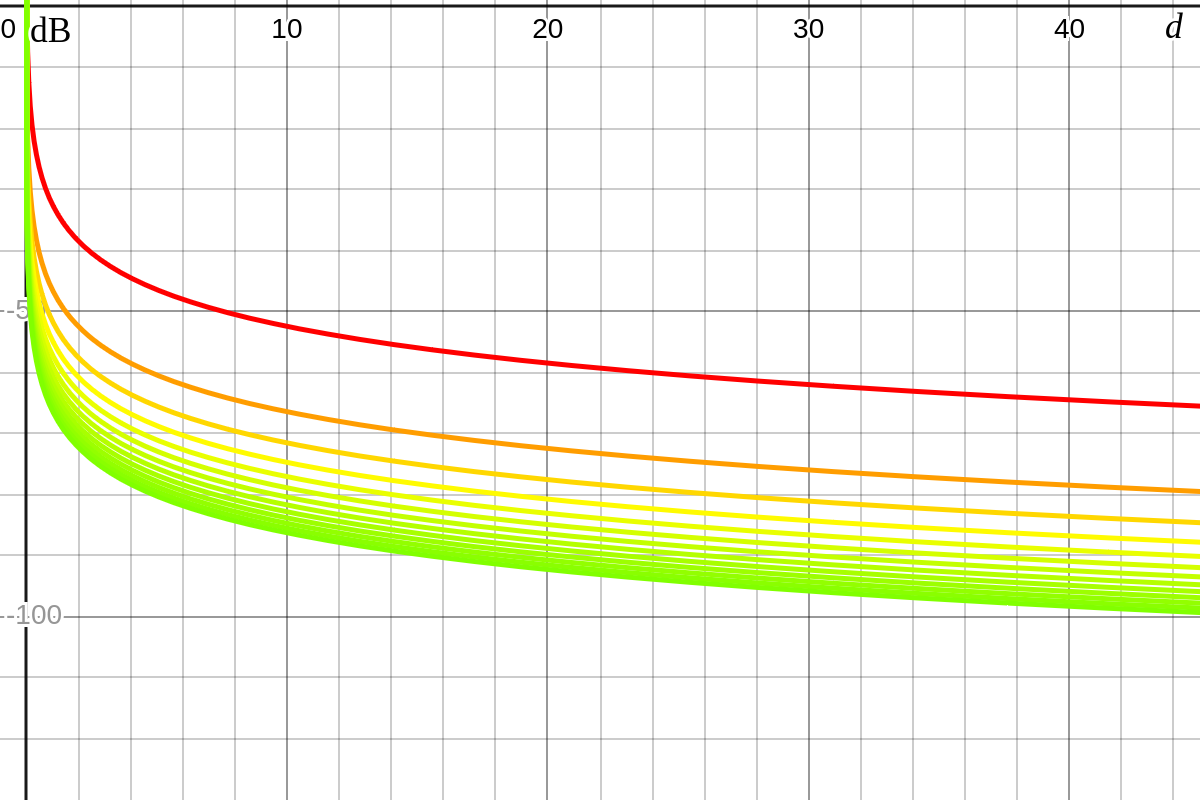
\includegraphics[scale=0.28]{../figures/friis.png}
\end{center}
I colori dal rosso al verde indicano 3 frequenze di trasmissione diverse:
$$
f = \left[3\cdot10^{9},\ 30\cdot10^{9},\ 300\cdot10^{9}\right]
$$
dove chiaramente la lunghezza d'onda si ricava come:
$$
\lambda = \frac{c}{f}
$$
dalla legge vista prima rispetto alle onde. Come vediamo, al crescere della frequenza (e quindi al diminuire della lunghezza d'onda) si ha che la potenza ricevuta sulla distanza diminuisce.

\subsubsection{Guadagno di antenna}
Le antenne in trasmissione e in ricezione possono concentrare le potenze in direzioni specifiche (e quindi diventare \textit{anisotropiche}, o direttive). Un antenna direttiva introduce un \textbf{guadagno} di antenna. Visto che abbiamo 2 antenne (trasmissione e ricezione) si ottiene una formula del tipo:
$$
P_r = \beta G_r G_t P_t
$$

Notiamo che il caso $G_r = G_t = 1$ equivale al caso \textit{isotropico}, visto prima.

\subsubsection{Array di antenne}
Un altro modo per incrementare la potenza ricevuta è quella di incrementare l'area aumentando il numero di antenne, magari usando una \textit{array} di antenne.

\par\smallskip

\noindent
\textbf{\textsf{Array sferiche}}

\noindent
Se si hanno $N$ antenne di superficie $A$ disposte in maniera sferica rispetto al trasmettitore, la potenza ricevuta $P_r$ aumenterà di $N$. Per riempire l'intera sfera di propagazione di antenne, avremmo bisogno di un numero di antenne pari a:
$$
N = \frac{4 \pi d^2}{A} = \frac{(4 \pi d)^2}{l^2} = \frac{1}{\beta}
$$
Questo è chiaro dal fatto che la relazione fra potenza ricevuta e trasmessa è:
$$
P_r = \beta P_t \cdot N
$$
per cui se $N = \frac{1}{\beta}$ si recupera tutta la potenza (ignorando il \textit{fading}).

\par\smallskip

\noindent
\textbf{\textsf{Array planari}}

\noindent
Nel caso di array disposte in maniera planare rispetto al trasmettitore, avremo che di base la potenza massima che potremo ricevere sarà quella ottenuta nell'ipotesi di una configurazione planare infinita:
$$
P_t = \frac{P_r}{2}
$$
dal fatto che solo un emisfero dei fronti d'onda trasmessi andrà ad incontrare il piano.

\subsection{Rapporto segnale-rumore}
Avevamo introdotto in 1.1.2 il concetto di rapporto \textit{segnale-rumore}, cioè di \textbf{SNR} (da \textit{Signal-Noise Ratio}). Di base, questo ci dà una metrica dell'informazione persa sull'antenna ricevuta, ed è:
$$
\mathrm{SNR} = \frac{P_r}{P_n} = \frac{\text{Potenza del segnale ricevuto}}{\text{Potenza del rumore termico}}
$$
dove una buona stima di $P_n$ é:
$$
P_n = B k_B T
$$
dove $B$ è la banda, $k_B$ la costante di Boltzmann, e $T$ la temperatura. Questo significa che all'aumentare della banda (quindi della frequenza $f$), la potenza del rumore aumenta e si ha più perdita di segnale utile.

Una volta noto $P_n$ possiamo riportarci alla forma più generale che abbiamo visto della legge di Friis (4.1), e cioè dire:
$$
P_r = G_r G_t P_t \frac{\lambda^2}{(4 \pi d)^2}, \ P_n = B k_B T \implies \mathrm{SNR} = G_r G_t P_t \frac{\lambda^2}{(4 \pi d)^2} \frac{1}{B k_B T}
$$
\begin{center}
	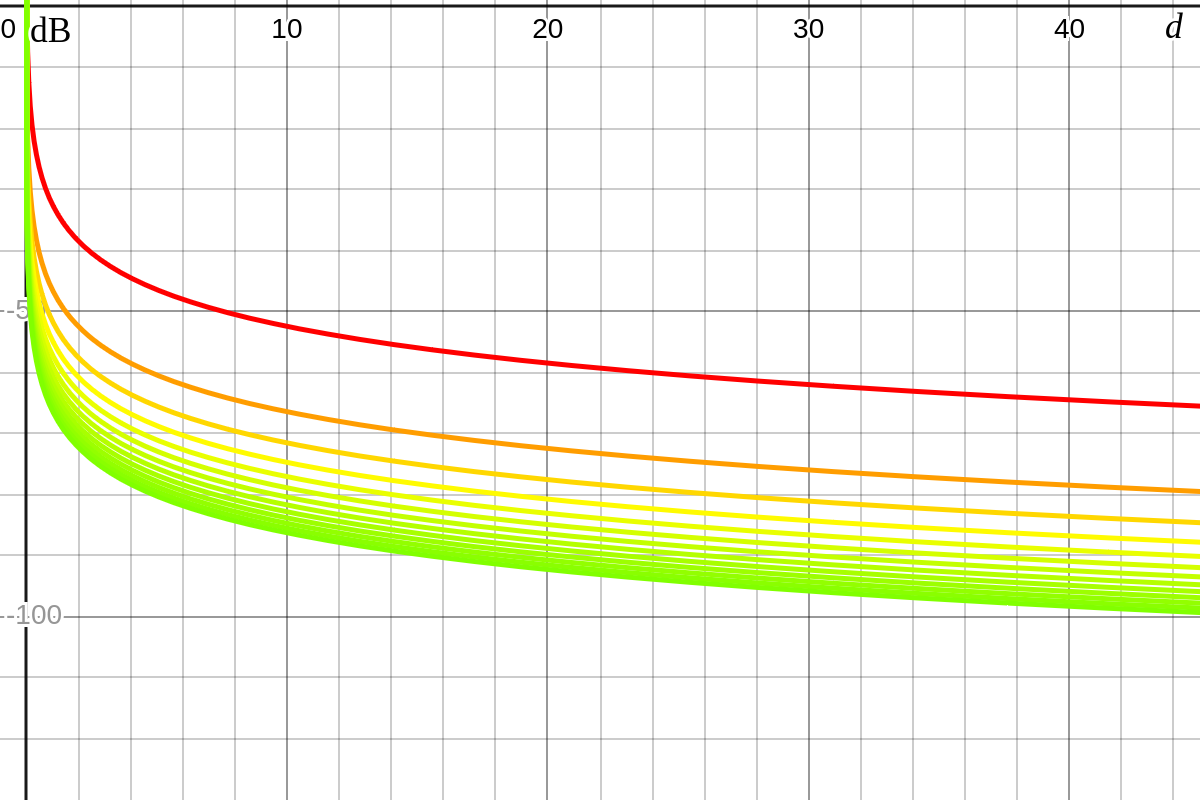
\includegraphics[scale=0.28]{../figures/friis.png}
\end{center}
Sulla distanza, quindi, mantenendo $T$ e $B$ costanti si ha che l'SNR si evolve come la potenza ricevuta $P_r$, cioè i rapporti segnale-rumore a basse distanze sono molto alti, per cui il segnale utile sovrasta il rumore sottostante. 

\end{document}
